\section{Исследовательский раздел}
В данном разделе была представлена постановка эксперимента, направленного на сравнение времени расчета турнирной таблицы в зависимости от двух факторов: количества команд, участвующих в турнире, и места проведения расчета, то есть на стороне базы данных или на стороне приложения. Для проведения эксперимента были подготовлены тестовые данные, включающая турниры с разным количеством команд и результаты матчей.

\subsection{Описание эксперимента}
В эксперименте сравнивается время расчёта турнирной таблицы в зависимости от количества команд в турнире и от используемой функции. Для каждого количества команд и каждой функции замеры производятся 10 раз, а затем вычисляется среднее арифметическое.

В листингах \ref{lst:res1} --- \ref{lst:res3} приведена реализация функции расчёта турнирной таблицы на стороне приложения.

\begin{lstlisting}[label=lst:res1,caption={Функция расчёта таблицы на стороне приложения (часть 1)}]
public IEnumerable<TeamStatistics> getTournamentTable(int tournamentId)
{
    List<TeamStatistics> table = new List<TeamStatistics>();
    IEnumerable<Team> teams = getTournamentTeams(tournamentId);
    foreach(var team in teams)
    {
        TeamStatistics statistics = new TeamStatistics(team.Name);
        IEnumerable<Match> matches = _matchRepository.getByHostTeam(team.Id, tournamentId);
        foreach(var match in matches)
        {
            statistics.Matches += 1;
            statistics.GoalsScored += match.HomeGoals;
            statistics.GoalsConceded += match.GuestGoals;
            if (match.HomeGoals > match.GuestGoals)
            {
                statistics.Wins += 1;
                statistics.Points += 3;
            }
            else if (match.HomeGoals == match.GuestGoals)
\end{lstlisting}
\begin{lstlisting}[label=lst:res2,caption={Функция расчёта таблицы на стороне приложения (часть 2)}]
            {
                statistics.Draws += 1;
                statistics.Points += 1;
            }
            else
            {
                statistics.Loses += 1;
            }
        }
        matches = _matchRepository.getByGuestTeam(team.Id, tournamentId);
        foreach (var match in matches)
        {
            statistics.Matches += 1;
            statistics.GoalsScored += match.GuestGoals;
            statistics.GoalsConceded += match.HomeGoals;
            if (match.HomeGoals < match.GuestGoals)
            {
                statistics.Wins += 1;
                statistics.Points += 3;
            }
            else if (match.HomeGoals == match.GuestGoals)
            {
                statistics.Draws += 1;
                statistics.Points += 1;
            }
            else
            {
                statistics.Loses += 1;
            }
        }

        table.Add(statistics);
    }
    table.Sort((y, x) =>
    {
        if (x.Points != y.Points)
        {
            return x.Points.CompareTo(y.Points);
        }
\end{lstlisting}
\begin{lstlisting}[label=lst:res3,caption={Функция расчёта таблицы на стороне приложения (часть 3)}]
        int xDiff = x.GoalsScored - x.GoalsConceded;
        int yDiff = y.GoalsScored - y.GoalsConceded;
        if (xDiff != yDiff)
        {
            return xDiff.CompareTo(yDiff);
        }

        if (x.Wins!= y.Wins)
        {
            return x.Wins.CompareTo(y.Wins);
        }

        return 0;
    });
    return table;
}
\end{lstlisting}

Реализация функции расчёта турнирной таблицы на стороне базы данных приведена в пункте 3.4.

\subsection{Результаты эксперимента}

Ниже приведены технические характеристики устройства, на котором выполнялось тестирование.

\begin{itemize}
	\item Операционная система: Windows 11 Home.
	\item Оперативная память: 8 Гб.
	\item Процессор: 11th Gen Intel(R) Core(TM) i5-1135G7 @ 2.40ГГц \cite{proc}.
\end{itemize}

Во время тестирования компьютер был нагружен только встроенными приложениями окружения, а также непосредственно системой тестирования.

В таблице \ref{res} приведены результаты эксперимента. Время в таблице измеряется в миллисекундах.
\newpage
\begin{table}[ht!]
	\centering
	\caption{Результаты сравнения времени расчёта турнирной таблицы в зависимости от количества команд и используемой функции}
	\label{res}
	\begin{tabular}{|p{3cm}|p{5cm}|p{5cm}|}
			\hline
			\textbf{Количество команд} & \textbf{Функция на стороне БД} & \textbf{Функция на стороне приложения}\\
			\hline
			10 & 11 & 101 \\
			\hline
			20 & 12 & 110 \\
			\hline
			30 & 12 & 222\\
			\hline
                40 & 14 & 320\\
			\hline
                50 & 16 & 475\\
			\hline
                60 & 17 & 547\\
			\hline
                70 & 19 & 632\\
			\hline
                80 & 21 & 746\\
			\hline
                90 & 23 & 850\\
			\hline
                100 & 25 & 958\\
			\hline
	\end{tabular}
\end{table}
На рисунке \ref{img:research} приведена зависимость времени расчёта турнирной таблицы в зависимости от количества команд и используемой функции.

\begin{figure}
  \centering
  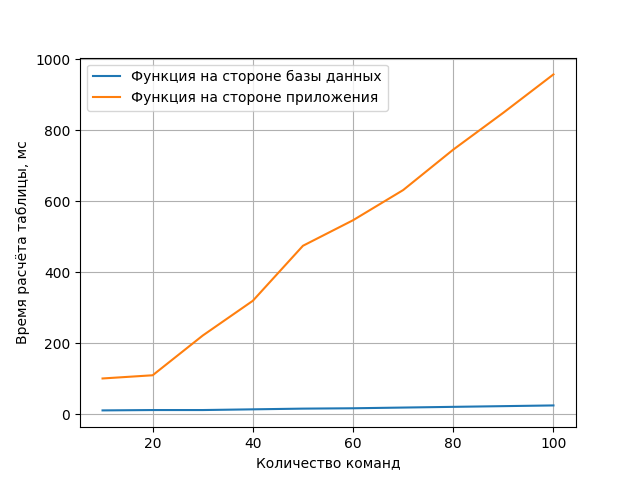
\includegraphics[scale=1]{inc/research.png}
  \caption{Зависимость времени расчёта турнирной таблицы в зависимости от количества команд и используемой функции}
  \label{img:research}
\end{figure}

\subsection*{Вывод}
В результате эксперимента было установлено, что время расчёта турнирной таблицы линейно зависит от количества команд, участвующих в турнире, вне зависимости от того, какая функция используется --- функция на стороне базы данных или на стороне приложения. Также выяснилось, что время расчёта таблицы при использовании функции на стороне приложения в $38,32$ раз дольше, чем при использовании функции на стороне базы данных при количестве команд, равном $100$.